\documentclass[12pt,a4paper]{article}

\usepackage[utf8]{inputenc}
\usepackage[english]{babel}
\usepackage{amsmath}
\usepackage{amsfonts}
\usepackage{amssymb}
\usepackage{graphicx}
\usepackage[left=3cm,right=3cm,top=3cm,bottom=3cm]{geometry}

\usepackage{hyperref}
\usepackage{caption}
\usepackage{subcaption}
\usepackage{mathtools}

\usepackage{listings}
\usepackage{color}
\usepackage{pgfplots}

\setlength{\parskip}{1mm}

\lstdefinestyle{scalasnp}{
	language=Scala,
	keywordstyle=\color{blue},
	frame = single,
	commentstyle=\color{black}
}

\lstdefinestyle{nirsnp}{
	language=sh,
	keywordstyle=\color{orange!50!red},
	frame = single
}

\author{Hugo Kapp 227942}
\title{Optimizations in the Scala Native compiler \newline \Large{Semester project report}}
\date{}

\newcommand{\scala}[1]{\textsf{#1}}
\newcommand{\nir}[1]{\texttt{#1}}
\newcommand{\perf}[1]{#1 \%}

\begin{document}

\maketitle

\section{Introduction}

We explain in this report what I have done during this semester project at LAMP, during the Fall semester 2016. We first explain what is the goal of this project, and why it important. We then describe briefly the specificities of the Scala Native compiler, focusing on ints intermediate representation (NIR). After this, we give the details of each optimization that was implemented. In section \ref{resultssection} we show the results observed over the codebase. After that, we briefly discuss what could be done in the future, before concluding.

\subsection{Motivation}

Because the goal of the Scala Native compiler is to produce binary executables from Scala source files, there can be no dynamic linking. This means that the techniques used in the JVM for late linking, i.e. loading classes when they are needed, at execution time, cannot be used. In Scala Native, the linking is done statically, and all the classes and methods that could be used during the execution are identified, then loaded at compile time.

This leads to very big programs that have to go through the whole compilation pipeline, making the compilation process slow, and outputting big LLVM source files. These are then compiled to large binary executables, containing portions of code that might never be used. The LLVM compilation of big files being slow, this slows down the compilation process even further. 

%In recent compilers, compilation speed is an issue. This is particularly important in Scala compilers, because the richness of the language is hard to resolve automatically. The process is therefore more complex, and thus, slower than for other languages.

%For ScalaNative, this problem is worsened by the long compilation time of LLVM, which is relatively slow when applied to big files. Because there can be no dynamic linking in ScalaNative, all symbols and definitions that can be reached during the execution of the program are statically linked during compilation. This produces very big programs that needs to go through the whole compilation pipeline.

%All of this makes the ScalaNative compiler very slow, and produces huge executables.

\subsection{Goal}

The goal of this project is to reduce the amount of code worked with, through various optimizations. We could let the LLVM compiler take care of this, as it has a very efficient optimization pipeline. The idea here is to take advantage of the domain-specific knowledge we have, like Scala semantics or code patterns, before it is lost due to primitives lowering to LLVM.

Because other metrics are hard to guarantee, measure and reason about, the only goal here will be code reduction. Reduction in the final size of the executable, compilation time or execution time is totally incidental, although always desirable.

\section{The Scala Native compiler}

% talk about the previous optimizations (DCE, boxing elimination, copy propagation)

Before we start explaining the various optimizations implemented and their impact, we first need to talk a little bit about the compiler organization and specifics. Only what will be necessary to understand the optimizations and the reason why they work is explained here, and kept abstract. For more details on the compiler, please refer to the documentation in \cite{nativedoc}.

\subsection{General organization}

The Scala Native compiler is a Scala compiler that outputs binary executables. It does so by using the LLVM language and compiler, a very powerful and broadly used cross-platform low level language, close to assembly \cite{llvmlang}.

The compiler is organized as a classic pipeline. After the front-end extracts the AST from the Scala source files, it goes through a sequence of lowering phases (called passes), which transforms the high-level constructs from Scala into low-level LLVM constructs, closer to assembly.

For this project, we only add passes to the compilation pipeline, which will alter the current form of the code.

\subsection{Native Intermediate Representation}

Scala Native uses its own intermediate representation (IR), called \textit{Native Intermediate Representation} and abbreviated NIR. This is the only form of the program on which we will work during this project.

The instruction set of NIR is composed of a subset of LLVM operations, with the same semantics, plus some high-level constructs coming from Scala (e.g. class definition, method dispatch, boxing...). The latter are lowered during the compilation process to be expressed in terms of LLVM instructions only.

Like LLVM, NIR uses the concept of \textit{basic blocks}, which is defined as a portion of purely sequential code. This means that the control flow cannot enter, nor exit in the middle of a basic block. In NIR, each basic block has a name and starts with a label, which defines the name of the block, as well as its parameters, and ends with a control flow instruction, which branches (potentially conditionaly) to another basic block using its name. For a given code, we then define the \textit{Control Flow Graph} (abbreviated CFG) as the directed graph whose nodes are the basic block of the program, with an edge going from block $n_1$ to $n_2$ if the control flow instructions of $n_1$ can branch to $n_2$. 

NIR programs are in SSA form (as is LLVM), which stands for \textit{Static Single Assignment}. This means that variables have only one static definition in the program. Note that this definition can be performed multiple times during the execution. Different values can then be merged to define a new variable, using the concept of $\phi$-functions that can be found in the litterature (see \cite{ssabook}). In NIR, classic $\phi$-functions are replaced by arguments passed to each basic block. Like in Scala, variables must be defined before their use.

% add a simple example !! for merging

All basic blocks, variables and control flow graphs are local to a given method, which are treated as complete programs, independent of each other. For the purpose of this report, we will write some basic NIR code, but won't bother with specific syntax of the language. However, we will keep the way variables are written, starting with a '\nir{\%}', e.g. \nir{\%a}. Further details about NIR can be found in \cite{nirdoc}.

\section{Global Value Numbering}

The first optimization implementend is called Global Value Numbering, and sometimes abbreviated GVN.

\subsection{Idea}

The idea is taken directly from \cite{ssabook}, which also provides a proof of correctness. The general idea is to reuse the result of computations that were already made in the past, which makes GVN a redundancy elimination optimzation. To be able to do that, two conditions need to be met :

\begin{enumerate}
\item The two computations yield the same result in all cases, and there is no side-effect
\item In all possible paths of the control flow, the result we want to reuse has been computed before the location we want to reuse it at
\end{enumerate}

The first condition is very simple to understand, but the second might seem more complex. It can be explained using the example in Figure \ref{fig:gvn}. In \ref{fig:gvn1}, the computation \scala{a + 1} is not necessarily done when we reach the definition of \scala{c}. In \ref{fig:gvn2}, the result has already been computed when we reach the definition for \scala{b}, so we can avoid the re-computation of \scala{a + 1}.

\begin{figure}
	\begin{subfigure}{0.5\textwidth}
		\begin{lstlisting}[style=scalasnp]
if (...) {
  val b = a + 1
  ...
}
val c = a + 1
		\end{lstlisting}
		\caption{Unreduceable code}
		\label{fig:gvn1}
	\end{subfigure}
	\quad
	\begin{subfigure}{0.5\textwidth}
		\begin{lstlisting}[style=scalasnp]
val c = a + 1
if (...) {
  val b = a + 1
  // val b = c
  ...
}
		\end{lstlisting}
		\caption{Reduceable code}
		\label{fig:gvn2}
	\end{subfigure}
	\caption{GVN examples}
	\label{fig:gvn}
\end{figure}

\subsection{Value Numbering}

Following its name, GVN uses value numbering to achieve the first condition. This is opposed to syntactic redundancy, where we consider that two expressions yield the same result only if they are written the same way (modulo the commutativity of operations).

In value numbering, each variable in the program has a hash value associated to it. We call the function that gives these hashes $h$. The hash value for variable $v$ is then given by $h(v)$. This value is computed using the defining operation for $v$, and the hash value for each of its operand. Note that this only works on programs that are in SSA form, like the NIR, because we need a single definition for each variable.

For example, say we have \nir{\%b = \%a + 1}. Then $h(\nir{\%b}) = h(\nir{\%a + 1}) = agg(\nir{+}, h(\nir{\%a}), h(\nir{1}))$. The aggregation function used ($agg$) is any hashing function.

Bootstrapping is done by giving each input variable a value that depend on its name. Constants are give a hash that depends on their value.

\subsection{Dominator tree}

To check for the second condition discussed earlier, we use the concept of dominator tree, also discussed in the SSA book \cite{ssabook}. From this very book, we get the following definition for domination :
\newline
A basic block $n_1$ \textit{dominates} basic block $n_2$ if every path in the control flow graph from the entry point to $n_2$ includes $n_1$. By convention, every basic block dominates itself.

In other words, $n_2$ is dominated by $n_1$ if we have to go through $n_1$ before going to $n_2$. Thus, if $v_1$ is defined in block $n_1$ and $v_2$ is defined in block $n_2$, and $n_1$ dominates $n_2$, then we know that the value of $v_1$ has been computed when we reach the definition of $v_2$. Note that this only holds if $n_1 \neq n_2$, but if it is the case, then it is trivial to check that $v_1$ is indeed defined before $v_2$.

We use this to build the dominator tree, which gives, for each block in the CFG, the set of blocks that dominate it. This allows us to easily check if the value of a variable $v$ can be used at a given point $p$ in the program, by verifying that $p$'s basic block is dominated by the block in which $v$ is defined.

\subsection{Algorithm}

Using both parts, we can then easily check which variables always have the same value, and reduce the ones computed later. The algorithm is as follows : \newline
For each instruction:
\begin{enumerate}
\item Compute the value for $v$, $h(v)$, using the values for its operands
\item For each variable $w$ that has the same value :
	\begin{enumerate}
	\item Check if the definitions for $v$ and $w$ match
	\item Check if the value of $w$ can be reused at $v$
	\item If both conditions are verified, then replace $v$ by $w$
	\end{enumerate}
\end{enumerate}

\subsection{Implementation}

Here we give a few details on the implementation on the described technique of Global Value Numbering.

First, we build the dominator tree by doing a single pass through the CFG. For each block $n_i$, the blocks dominating it is the set $D_i = \{i\} \cup \left( \bigcap\limits_{j \in pred(i)} D_j \right)$, where $pred(i)$ gives the set of predecessors to the block $n_i$ in the CFG. When the CFG contains loops, we need to do a fixpoint to find the correct domination set.

We use the \textsf{Murmur3} hash function, from the scala standard library (\scala{scala.util.hashing.MurmurHash3}). This provides good and very fast hashes, which is useful because we don't need cryptographic-level hashing. We take 32 bits hashes because it is convenient (it allows us to use the \scala{hashCode} function whenever possible), and is enough not to produce collisions (false positives, discussed later).

Even with hashing done correctly, we still need to define what it means for two variables to have the same definition. This is done in a recursive manner, using the following rules :
\newline
Two variables $a$ and $b$ are \textit{deep equal} if:
\begin{enumerate}
\item $a$ and $b$ have the same name (they are indeed the same variable)
\item or their respective definitions match, i.e. they use the same operation, and their operands are \textit{deep equal}
\end{enumerate}

Having defined all of this, we just follow the algorithm sketched above, building the dominator tree before going through the code. Note that, when a variable $b$ is found to be replaceable by the value of another variable $a$, we use a simple NIR instruction \nir{copy}, which avoids having to replace $a$ by $b$ everywhere (\nir{copy} instructions are simplified later in the pipeline).

\section{Control-flow optimizations}

We discuss in this section various optimizations that are aimed at simplifying the control-flow graph.

\subsection{Unit simplification}

\subsubsection*{Problem}

In Scala, every code block has a value. This is very useful in general, but sometimes the value is not used. Nevertheless, it has to be accounted for by the compiler, that the value of this block might be used later in the future. This is especially true for if-then-else blocks, where the value is usually not important. In such cases, the types of the last instruction of the said blocks rarely match, or match with unit (with assignment variables for example).

% the case is actually if alone (no else) !

In this case, the Scala Native compiler still needs a way to merge the outcomes of these code blocks, and does so by having the next basic block have a parameter of type \scala{Unit}, where the two branches give their own output value. This is shown in Figure \ref{fig:cfc}. This is not necessary, as we know that \scala{Unit} is the type that has only one value (the \scala{Unit} object).

\subsubsection*{UnitSimplification}

To solve this problem, we add a very simple pass to the compiler, called \scala{UnitSimplification}. Its job is very simple : whenever a variable of type \scala{Unit} is used (either as an operand, or given as a parameter to a block or function), it is replaced by the actual value \scala{Unit}.

This is helpful because the LLVM compiler can not simplify all of these variables later, because it doesn't know that the type \scala{Unit} only has one value. But this alone wouldn't be enough.

\subsubsection*{Dead parameters elimination}

Simplifying the unit usage is a nice thing, but it still leaves a complicated CFG, with a lot of unused block parameters. Even if the parameter variable with type \scala{Unit} was indeed used in the block, its use gets replaced by the value \scala{Unit}. Therefore, all block parameters with type \scala{Unit} can be removed.

We can actually generalize this by adding to the normal \scala{DeadCodeElimination} phase a simple analysis on the block parameters on top of the normal variables. This simplifies the CFG a lot, and makes it more readable.

Note that these improvements do not reduce the code size by themselves (not in terms of code lines at least), but allows for further optimizations in the other passes, and increases the optimization potential of LLVM as well.

\subsection{Control-flow chains}

\subsubsection*{Problem}

The original CFG produced by the compiler is very simple. For any control-flow branching, it produces a "diamond", which is the result of the left branch and right branch dissociating, then merging in the next shared portion of the code. But in many cases, this is not necessary.

For example, take the code in Figure \ref{fig:cfc} and its (simple) CFG. Because there is no "else" part to the "if", we could already jump to the block \nir{\%src.5} without going through \nir{\%src.4} if the condition is not met.
% This goal CFG is shown in \ref{fig:cfc:cfg2}.

\begin{figure}
	\begin{subfigure}{0.5\textwidth}
		\begin{lstlisting}[style=scalasnp]
if (...) {
  println(..)
}
// no else
		\end{lstlisting}
		%\caption{Simple example code}
		%\label{fig:cfccode}
	\end{subfigure}
	\quad
	\begin{subfigure}{0.5\textwidth}
		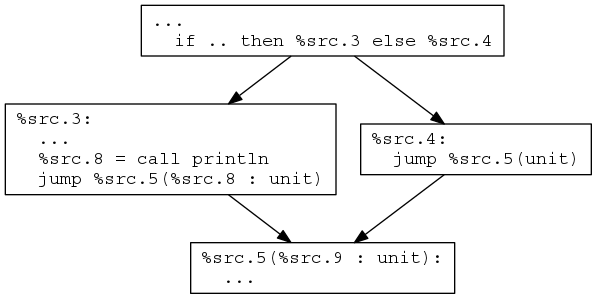
\includegraphics[width=\textwidth]{images/cfc-cfg1.png}
		%\caption{Reduceable code}
		%\label{fig:cfccfg1}
	\end{subfigure}
	\caption{A simple code example, and its corresponding CFG}
	\label{fig:cfc}
\end{figure}

\subsubsection*{CfChainsSimplification}

To solve the kind of problems explained above, we add a new pass to the compiler, called \scala{CfChainsSimplification}. Its goal is to simplify the control flow using global CFG informations, and in particular to solve these simple control-flow chains, where a block is only comprised of a single control-flow instruction. We use the following rules for simplification :

\begin{figure}
$$ \frac{\nir{\%a(\%b..): Cf}}{\nir{jump \%a(\%c..)} \longrightarrow \nir{Cf} \  | \  \{\nir{\%b..} \rightarrow \nir{\%c..}\}} $$

$$ \nir{if true then \%a(\%b..) else \%c(\%d..)} \longrightarrow \nir{jump \%a(\%b..)} $$

$$ \nir{if false then \%a(\%b..) else \%c(\%d..)} \longrightarrow \nir{jump \%c(\%d..)} $$

$$ \frac{\nir{jump \%a(\%b..)} \longrightarrow^* \nir{jump \%a'(\%b'..)} \quad \nir{jump \%c(\%d..)} \longrightarrow^* \nir{jump \%c'(\%d'..)}}{\nir{if \%e then \%a(\%b..) else \%c(\%d..)} \longrightarrow \nir{if \%e then \%a'(\%b'..) else \%c'(\%d'..)}} $$

$$ \nir{switch \%a \{ default: \%b \} } \longrightarrow \nir{jump \%b} $$

$$ \frac{\nir{\%a = \%b}_i}{\nir{switch \%a \{ cases \%b..: \%c.. ; default: \%d \} } \longrightarrow \nir{jump \%c}_i} $$

$$ \frac{\nir{jump \%c}_i \longrightarrow^* \nir{jump \%c'}_i \quad \nir{jump \%d} \longrightarrow^* \nir{jump \%d'}}{\splitfrac{\nir{switch \%a \{ cases \%b..: \%c.. ; default: \%d \} }}{\longrightarrow \nir{switch \%a \{ cases \%b..: \%c'.. ; default: \%d \} }}} $$
\centering
\end{figure}
\hspace{2mm}

\textit{Where} \nir{Cf} \textit{is any single control-flow instruction.}

\hspace{2mm}

The pass does fixpoint iterations on each control-flow instruction, following the rules above, until convergence for this instruction has been reached. This is particularly useful when the control flow chains are rather long, and static information is carried along (for example a \nir{jump true} that jumps to an \nir{if} can directly be reduced).

\subsection{Merging basic blocks}

\subsubsection*{Idea}

A very simple control-flow simplification is the one that reduces unnecessary basic blocks. The conditions for a block $n_1$ to be removed is that is has only a single predecessor in the CFG $n_p$, and $n_p$ must have a single successor in the CFG. In this case, we can merge the two blocks into one, because we know the control flow will always go to $n_1$ at the end of $n_p$, and $n_1$ is not used anywhere else.

This is an easy way to reduce the CFG and the number of branching that appear in the code. On top of that, because the parameters of the fused block now have known values, additional optimizations may trigger, simplifying the code further.

\subsubsection*{BasicBlocksFusion}

For this implementation, we add a new pass called \scala{BasicBlocksFusion}, which fuses together blocks that satisfy the aforementioned conditions.

\subsection{Reducing block parameters}

\subsubsection*{Problem}

Even after the passes described above have been executed, there is still information that can be extracted from the CFG and be made explicit. We talk here about block parameters that are always supplied the same argument. We can simplify these by removing the said parameter, and replacing it by its supplied value. This simplifies the CFG, because blocks have less parameters, and makes their value explicit, allowing further optimizations to trigger.

\subsubsection*{BlockParamReduction}

Once again, we add a new pass, called \scala{BlockParamReduction}. First, it gathers the argument values that are supplied to each block parameter in the CFG. Then, parameter \nir{\%a} is removed if the set of supplied values has a single value, not counting the recursive value \nir{\%a}. We then remove the arguments from the branching locations. All of this can be done in three passes : one to build the CFG, one to gather the arguments, and one to simplify the branching and the parameters.

\section{Static evaluation}

We discuss here various static evaluation and pattern-based optimizations.

\subsection{Canonicalization}

% inspired by LLVM

\subsubsection*{Goal}

Because the partial evaluation and instruction combine passes are pattern-based, and some of these pattterns depend on the presence of static values (i.e. not variables), we perform canonicalization first. The goal of canonicalization is to simplify the writing of patterns, by ensuring an invariant on their location. We use here the same convention as in the LLVM compiler, and say that any static value that can be moved, is moved to the right operand. This means we only move operands for commutative operations.

\subsubsection*{Canonicalization}

The \scala{Canonicalization} pass is very simple. For each instruction, if it is commutative and has a static operand, then it is moved to the right-hand side.

This only makes sense to perform on binary operations. The only such instructions in NIR are arithmetic, logical and comparison operators. All of these are also LLVM instruction, with the same semantics. Because LLVM has a very efficient optimization pipeline, the goal here is not to do better than the underlying compiler, but to extract simple statically known information that might be useful for the other optimization passes (which use domain-specific knowledge).

Note that we do not modify instructions that manipulate floats (these are explicit instructions), because float handling is too complicated for the purpose of this project. We therefore let all float-instructions optimization to LLVM. We prefer safety over mis-optimization.

\subsection{Constant folding}

\subsubsection*{Idea}

Constant folding is very simple. It basically emulates the run-time output of each instruction that has all its operands statically known. We can therefore propagate the knowledge we have further in the code.

This is simple, but needs to capture perfectly the semantics of each operation. Most of them can easily be performed in Scala, but some of the low-level instructions may be hard to express in such a high-level language.

Here again, we do not do anything with float instructions, to make sure we keep the semantics of the original program intact.

\subsubsection*{ConstantFolding}

We add a pass called \scala{ConstantFolding}. Because it needs all its operands to be static, it is not dependent on the \scala{Canonicalization} pass. This pass is only concerned with low-level instructions, because high-level instructions with static values are optimized in their own lowering pass. This is then a trivial pass, but special care has to be taken to follow the semantics of the LLVM operators.

\subsection{Partial evaluation}

\subsubsection*{Idea}

The idea of partial evaluation is to use simple rules to simplify single instructions that have some static information. An example would be to say that $a \times 0$ can always be replaced by the value $0$, irrespective of the value of $a$.

Such optimization passes are a set of patterns which, when they apply to the current input, need to simplify the code in some way or another. The code reduction is an obvious target, but not necessarily the best. One can easily devise a (potentially abritrary) total ordering on the set of instructions, and say that the lower instructions are simpler. In this case, reducing the code size, or bringing an operation down in the ordering are acceptable simplifications.

Making sure that each pattern actually simplifies the code is important. It may provide a  very easy check for useless patterns, but also ensures that a fixpoint method will always converge.

\subsubsection*{PartialEvaluation}

We add yet another pass to the compiler, called \scala{PartialEvaluation}. It is a list of single-instructions patterns that all simplify the code. The ordering over the instructions can easily be devised, and is relatively intuitive, but is not detailed here. Because using a \nir{copy} operation is effectively reducing the code size, it is quite obvious that the \nir{copy} instruction is at the bottom of this ordering.

\subsection{Instruction combine}

\subsubsection*{Idea}

The idea for this optimization is inspired by the LLVM pass called \scala{InstCombine} \cite{llvmpasses}. Relatively close to partial evaluation, this pass goes further and simplifies patterns that use knowledge about variable definitions. It is therefore able to capture patterns that span mutliple instructions.

\subsubsection*{InstCombine}

We add a pass called \scala{InstCombine}. Its role is to simplify multi-instructions patterns in the code. Very close to partial evaluation, it is however distinct, because it deals with much more involved patterns, and doesn't require the operands to have statically known values. It uses the operation defining its variable operands to perform optimizations.

\begin{figure}
	\begin{subfigure}{0.5\textwidth}
		\begin{lstlisting}[style=nirsnp]
%a = ...
%b = xor %a, true
if %b then %c else %d
		\end{lstlisting}
		\caption{Raw code}
	\end{subfigure}
	\quad
	\begin{subfigure}{0.5\textwidth}
		\begin{lstlisting}[style=nirsnp]
%a = ...
%b = xor %a, true
if %a then %d else %c
		\end{lstlisting}
		\caption{Optimized code}
	\end{subfigure}
	\caption{A code pattern simplifiable by instruction combine (NIR code)}
	\label{fig:ic}
\end{figure}

An example that occurs a lot in the produced code is shown in Figure \ref{fig:ic}. The \nir{xor} with the value \nir{true} is used to negate a boolean value, as LLVM doesn't have a negation opertator. This code is the result of a simple '\scala{if (!a)}' expression in the original scala code. We can avoid computing the intermediate value \nir{\%b} by simply switching the branching destinations. Note that the optimized version of the code does not get rid of the definition for \nir{\%b}. This is because it could be used somewhere else in the code, although this is unlikely. Anyway, it will be cleaned up by the dead code elimination pass if possible.

The criteria for reducing code is thus more complex than the one used in the last section. Here, on top of reducing instructions to simpler ones, we can also reduce the number of variable used. This may lead to some variables being reomved by DCE, which eventually reduces the code size. 


% need a note on passes placement

% add examples everywhere !

\section{Results}

\label{resultssection}

We discuss in this section the impact the optimizations mentioned in the above sections had.

\subsection{Methodology}

We here describe the methodology used to measure the impact of the optimization, as well as the metrics used : how they are computed, and how they can be interpreted.

\subsubsection{Code base compilation}

\label{codebase}

The linker of the Scala Native compiler gathers all the code that is potentially reachable from the main program given. Because it is hard to produce a program that reaches the maximum number of classes and methods possible, we bypass the linker. We create a routine that gathers all symbols (classes and methods) in the entire code base, and run the compilation passes on this code.

The code base is the product of all the code that is pre-compiled and kept in \texttt{.nir} files. It is composed of the entire Scala library, a specific Scala Native library, as well as the parts of the Java library that have been re-implemented in Scala for the purpose of Scala Native. We also have some other programs and benchmarks.

The entire code base described here contains, as of January 3rd, 2017, 5195 compiled files, for a total of 588'295 lines of NIR code. However, because the Scala library has some dependency on the Java library, and that the latter is not complete, some of the files have to be disabled. This leads to a valid codebase of 210'228 lines of NIR code. This will give a reasonable approximation of the impact the added pass have on general purpose code, due to the size and diversity of goals for the different code sources.

\subsubsection{Metrics}

We detail here the various metrics used to measure the performance achieved by the implemented optimizations. We also interpret the results, explaining their meaning and showing why one could expect different results.

\subsubsection*{Raw code reduction}

The first, and most obvious metric, is the raw code reduction. Mostly shown as a percentage of line reduction, it is sometimes used as the raw number of lines removed by the various optimization phases.

\subsubsection*{Optimizeable code reduction}

An extension of the previous criterion is called \textit{optimizeable} code reduction.

The problem with the raw code reduction is that it doesn't take into account what could have been changed, and what has to be fixed. For example, all the global definitions that have to be there (NIR declares classes and traits separately from the methods they define). All of these cannot be reduced. On top of that, each method needs to have a first line of declaration, an entry block label, at least one control flow instruction, and a closing brace.

Using this knowledge, we define the optimizeable code of some program as :

$$ opt(p) = \sum\limits_{m \in methods(p)} size(m) - 4 $$

This gives us a metric that takes into account how reduceable the code actually is.

\subsubsection*{Touched methods}

One other way to think about the changes the optimizations added have on the codebase is to see how many methods it affects, and out of these, what is the code reduction. This is also useful to show the impact of the very few passes that do not reduce the code size (e.g \scala{UnitSimplification}).

We use this criterion to derive another metric, which is the proportion of reduced code among the touched methods. This will allow us to compare the performance of passes that have the same raw reduction, but behave very differently : they either touch a lot of methods and have small changes on all of them, or touch very few, but have a big impact on these.

% add std-dev for code reduction out of touched methods

\subsection{Observed results}

We show here the results observed on the code base described in \ref{codebase}, in terms of code reduction, using the metrics discussed above.

\begin{table}
	\centering
	\begin{tabular}{| l | r | r | r | r |}
\hline
                  & Raw         & Optimizeable & Touched     & Out of touched \\ \hline
GlobalValueNumbering & \perf{0.47} & \perf{0.99}  & \perf{5.66} & \perf{2.13} \\ \hline
UnitSimplification & \perf{0} & \perf{0}  & \perf{7.55} & \perf{0} \\
CfChainsSimplification & \perf{4.26} & \perf{8.94}  & \perf{4.74} & \perf{20.97} \\
BasicBlocksFusion & \perf{0.91} & \perf{1.91}  & \perf{5.11} & \perf{4.33} \\
BlockParamReduction & \perf{0} & \perf{0}  & \perf{0.52} & \perf{0} \\ \hline
Canonicalization & \perf{0} & \perf{0}  & \perf{0.98} & \perf{0} \\
ConstantFolding & \perf{0.04} & \perf{0.07}  & \perf{0.23} & \perf{2.22} \\
PartialEvaluation & \perf{0.06} & \perf{0.12}  & \perf{0.4} & \perf{2.24} \\
InstCombine & \perf{0.1} & \perf{0.21}  & \perf{0.79} & \perf{2.72} \\ \hline
All combined & \perf{6.46} & \perf{13.35}  & \perf{13.28} & \perf{22.07} \\ 
\hline
	\end{tabular}
	\caption{Code reduction achieved by each pass}
	\label{restable}
\end{table}

Table \ref{restable} shows the measurement for all the individual passes, tested in isolation, as well as the results when we put all the optimization phases one after the other, in the order described in this report (except \scala{GlobalValueNumbering}, which comes last). The placement of passes is described more in detail in the next section.

We can clearly see here that \scala{CfChainsSimplification} is an outlier, in terms of code reduction. That is because it is fairly easy to simplify the simple, yet very verbose control flow graph that is outputted by the first phases of the compiler. For example, the pattern shown in Figure \ref{fig:cfc} happens very often : once for every \scala{if} that doesn't have an \scala{else}. On top of reducing the code size, this kind of simplification is good for runtime performance and other analyses of the code, because we have a simpler control flow, with less branching.

Global value numbering and blocks fusion give convincing results. Static code optimizations are in general very hard, because of the limited amount of information accessible. On top of that, one has to be very careful not to change the semantics of the original program. Therefore, these kinds of optimizations have a limited impact, except if the code base or the previous phases have specific recurring patterns (as in \scala{CfChainsSimplification}. Between 1 and 2\% (optimizeable) code reduction is in the bounds of results that are found to be satisfactory in the litterature.

Now, one can also see that the impact of the pattern-based optimizations, as well as constant folding, is very limited. They touch very few methods, and change only a couple of lines in each of these (1 out of 50). This can be expected for high-level languages like Scala, because constants are pretty rare. Good code practice encourages the use of parameters and defined constants, thus "hardcoding" of values happens very rarely, leading to poor optimization performances for passes that require statically known values. Note that the most applied patterns in these are actually produced by the earlier phases of the compiler.

The number of methods touched help us measure the impact of non-code reducing optimizations. This is important when we put everything together, because these phases help the other phases find suitable patterns, leading to improved code reduction overall.  For the same reason as explained above, the canonicalization phase and the block parameter reduction trigger rarely. On the other hand, unit simplification happens a lot : it applies in 1 out of 13 methods. This is very useful because it reduces the passing of arguments in the control flow, which, for \scala{Unit}, is not optimized very well by LLVM, but also reduces the number of parameters that some basic blocks have. This simplifies the conditions for the control flow based optimizations, leading to more code reduction.

When we test all the phases together, we get a result that is slightly greater than the sum of the separate passes (\perf{13.35} vs \perf{12.24} on optimizeable code). This is due to the interconnection of the phases, simplifications incurring other simplifications.


\subsection{Pipeline integration}

In the previous section, we showed the code reduction for the implemented passes, without complete integration into the compiler pipeline. We discuss here what changes, and how / where to place the passes. Note that the compilation here is not done on the codebase anymore, as we need information from the linker here. We compile on our set of benchmarks instead, derived from the Scala-JS benchmarks \cite{scalajsbench}. It has a total of 7136 lines of Scala code, resulting in 105392 lines of NIR.

Passes placement is in general a very hard problem. Because some phases may create opportunities for other, but also potentially remove some opportunities, this is non trivial. Some placement invariants are relatively simple to figure out (for example, canonicalization needs to be done before partial evaluation and instruction combine). Apart from that, heuristics are hard to find because of all the intricacies of the different passes. Automatic placement has been tested, but no improvement could be achieved.

However, two things can increase the total code reduction. One is to try to place the optimization before or after the lowering phases of the compiler (or both). The other thing to do is what we will call \textit{knowledge propagation}, i.e. use copy propagation and dead code elimination extensively between the passes.

First, let's consider the placement of the optimizations in the compilation pipeline. One could argue that placing them before is a good idea, because the code is still high-level, and Scala code patterns can be found and eliminated here. But one can also argue for the opposite, i.e. placing the optimizations at the end of the pipeline, because the code transformations used for lowering also exhibits patterns that are easy to simplify. Because there are arguments for (and against) the two, both have to be tested. We also test both at the same time, and analyze the impact on the compilation time in the next section. Finally, we try, for each pass, if it should be before or after the lowering phases. This will give (hopefully) a good trade-off between compilation time and code reduction.

We also try \textit{knowledge propagation}, which consists in eliminating \nir{copy} instructions and dead code as soon as possible. The fact that code is not really removed in any optimization pass, but replace by \nir{copy} instruction is easier to write and verify (because the variable is still there). However, this also blocks optimizations opportunities, because it doesn't reflect the fact that the value of some variables is statically known. The same is true with dead code, except for the fact that it is not known at that time that some variables become dead after optimization. The idea here will be to add copy propagation and dead code elimination between almost all of the passes. This increases the compilation time, and is discussed in the next section.

\begin{figure}
	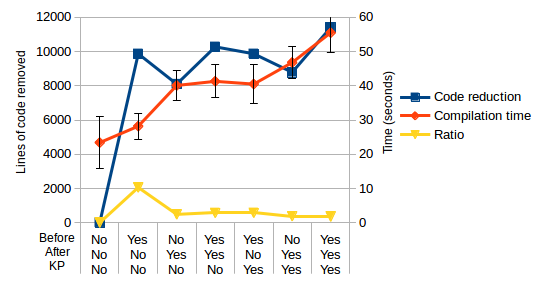
\includegraphics[width=1.15\textwidth]{images/integration-side.png}
	\caption{Comparison of the different placement for the optimizations (\textit{Before} and \textit{After} the lowering phases), as well as with or without knowledge propagation (\textit{KP}). For compilation time, we give the average over 10 runs as well as sandard deviation. The ratio, given in lines of code per second, is computed as $\frac{code\ reduction}{t - t_{ref}}$}
	\label{fig:pipinteg}
\end{figure}

Results for all the variants of the pipeline discussed are shown in Figure \ref{fig:pipinteg}. We can see that the performance is better if we perform optimization before lowering (more code reduction, and less compilation time). The change in compilation time is mostly due to the handling of a more complex CFG, with more nodes and more branching. The code reduction improvement validates the argument that the optimizations should be performed before lowering because of the code being high-level, allowing the finding of patterns and gathering of information to be much simpler.

We can also see that adding knowledge propagation only improves the results by a small amount (\perf{6.5} on average), but increases the compilation time substantially (\perf{+31.5} on average). The best system overall for code reduction, without taking into account the added compilation time, is obviously the one that has both optimizations before and after lowering phases, plus knowledge propagation. However, if we look for a good trade-off, then we can look at the \textit{ratio} shown on the graph : it gives the number of code lines removed per added second of compilation time. They are all relatively low (between 355 and 580 LOC/sec), except for the very first pipeline, which achieves 2050 LOC/sec. This is due to an almost optimal code reduction (\perf{86} of the optimal), with only \perf{20.5} added compilation time. We therefore use this specific placement in the real compiler.

\subsection{Other impacts}

We discussed in earlier sections code reduction, which was the main goal for this project, and also compilation time, which, although not a major goal, is important to keep low for performance of the compiler. We now talk about other impacts of the added optimizations, namely final executable code, which will show the LLVM optimizations that were enabled, and execution time.

% executable size difference !

% compile without the reporter !!

% give the specs fo the CPU

\section{Future work}

Static optimizations is a never-ending work. There are always patterns to add, new patterns added by other changes to the compiler, opportunities emerging from the combination of multiple phases ... However, some new optimization might have a big potential of code reduction.

First of all, inlining would be very interesting. Because the optimizations added use static local knowledge that is derived from the code, inlining methods would allow the knowledge about the parameters to "transfer" to the method implementation. Also, because of the way Scala code is written, i.e. typically with a lot of very small methods, with simple control-flow, the overhead of inlining in terms of added code can quickly be overcome	 by the simplifications that arise and the removal of a method call. However, this can't be applied to virtual methods, which happen to have a lot of methods that return constant, statically-known values. On top of that, good criteria to decide which methods to inline, and when to stop inlining are hard to devise.

One other optimization that could produce good results is the family of optimizations called "code motion". Their goal is to move code around, in order to execute instructions as soon as possible, if we know that we will compute them, or as late as possible, if thy might not be useful right away. One example is partial redundancy elimination, which, close to global value numbering (which is a full redundancy elimination method), tries to share values that are computed and used in various branches. This kind of optimizations i really hard in general, but some basic version could help a lot. By looking at the NIR code, one can see plenty of basic blocks that do the exact same thing, except for a variable name being different (or some value say). These blocks could be merged together, and a block parameter added to reduce the code (at the cost of potentially lost information for other passes). Also, there are many blocks with a conditional branch, for which all the children perform the same first instructions. Here, we could move this code in the current block, and perform branching later. However, these are hard to implement, and it is not easy to find good ways to find which code can be moved, and even harder to say if it should be moved.

% individual pass tests for correctness

\section{Conclusion}

During this project, many optimizations for NIR code have been implemented. It has later been shown that they produce convincing results in terms of code reduction, without slowing the compilation process very much.

We have seen that optimizations that have domain-specific knowledge, either through higher-level instructions or using specific patterns produced by the earlier phases, are the ones that reduce the code the most. On the other hand, very general-purpose optimizations, that are not very compiler or language specific, perform poorly (e.g. \scala{InstCombine}, \scala{PartialEvaluation}). This goes to show that the code that needs to be optimized must be known before thinking about which optimizations to implement.

\section*{Acknowledgements}

I would like to thank Martin Odersky for letting me the opportunity to do a semester project in his renowned lab, and in the very specific domain of compilers.

I would also like to thank Denys Shabalin for his deep interest in research and the help he provided me throughout this project.

I would also like to thank Doeraene Sébastien for his incredible knowledge about Scala compilers, and providing us with help, ideas and experience from his own Scala-JS project.

\begin{thebibliography}{9}

   \bibitem{nativedoc} Scala Native documentation \newline \url{http://scala-native.readthedocs.io}

	\bibitem{nirdoc} NIR documentation \newline \url{http://scala-native.readthedocs.io/en/latest/contrib/nir.html}
	
	\bibitem{ssabook} SSA book
	
	\bibitem{llvmlang} LLVM language reference \newline \url{http://llvm.org/docs/LangRef.html}	
	
	\bibitem{llvmpasses} LLVM compiler passes \newline \url{http://llvm.org/docs/Passes.html}

	\bibitem{scalajsbench} Scala JS benchmark \newline \url{https://github.com/sjrd/scalajs-benchmarks}

\end{thebibliography}


\end{document}